\section{Matrix Multiplication with MPI}

\begin{itemize}

    \item {
        \textbf{병렬화 방식.}
        \texttt{matmul} 함수는 입력 행렬을 각 프로세스에 분배하고, 각 프로세스가 할당받은 행렬을 사용하여
        행렬곱 연산을 수행한 뒤, 결과로 얻은 행렬을 root 프로세스에 모으는 방식으로 구현하였다.

        입력 행렬 A는 \texttt{MPI\_Scatter}를 사용하여 각 프로세스에 각기 다른 row들을 분배하였다.
        주어지는 입력의 특성상 행렬 A의 크기가 B에 비해 크기 때문에, A의 전체가 아닌 일부만을
        다른 프로세스에 전달하도록 구현하였다.

        입력 행력 B는 \texttt{MPI\_Bcase}를 사용하여 행렬 전체를 나머지 모든 프로세스에 전달하였다.
        이를 통해 각 프로세스는 행렬 C의 일부분을 모두 계산할 수 있게 된다.

        마지막으로 \texttt{MPI\_Gather}를 사용하여 각 프로세스가 계산한 행렬 C의 일부분을 root 프로세스에
        모으도록 구현하였다.

        한 프로세스에서는 OpenMP를 사용하여 연산을 병렬화하였다.
        주어진 행렬은 row-wise 방식으로 메모리를 사용한다는 점 (바로 다음 메모리가 같은 row의 다음 element) 을
        고려할 때 행렬 B를 쪼개는 것이 할당된 행렬 A에 대한 캐시 활용도를 높일 수 있을 것이라고 판단하였다.
        이에 각 thread가 할당된 행렬 A를 모두 사용하고 행렬 B의 일부 column을 사용하여 행렬 C의 일부 column을
        계산하도록 코드를 작성하였다.

        계산 중간에 thread 사이의 synchronization은 일어나지 않으며, 각 thread의 계산이 끝나는
        시점이 균일하도록 각 thread에게 행렬 C의 column을 균등히 할당하였다.
        
        또한, 한 번에 행렬 C의 $64 \times 64$ 만큼을 계산하도록 하는 macro kernel을 정의하여
        연산 과정이 cache-friendly 하도록 하였다. Macro kernel 내부에서는 AVX512 intrinsic 코드를 사용하여
        연산을 가속하였다.
    }
    
    \item {
        \textbf{최적화 방법 및 고려 사항.}
        성능 최적화를 위해 고려한 점에는 다음과 같은 것들이 있다.
        \begin{itemize}
            \item 통신 최적화를 위해 비교적 크기가 큰 입력 행렬 A를 쪼개어 각 프로세스에 전달하도록 구현하였다.
            \item OpenMP를 사용하여 연산을 병렬화하는 과정에서 thread 사이의 synchronization이 일어나지 않도록 구현하였다.
            \item Macro kernel을 정의하여 연산 과정이 cache-freindly하도록 구현하였다.
            \item SIMD 명령어인 AVX512 명령어를 사용하여 여러 연산이 한 번에 일어나도록 구현하였다.
        \end{itemize}
    }
    \item {
        \begin{figure}[t]
            \centering
            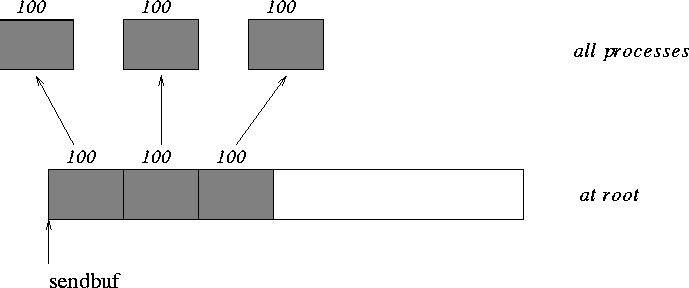
\includegraphics{imgs/mpi_scatter.png}
            \caption{\texttt{MPI\_Scatter}의 작동 방식\cite{MPIScatter}.}\label{fig:mpi_scatter}
        \end{figure}
        \begin{figure}[t]
            \centering
            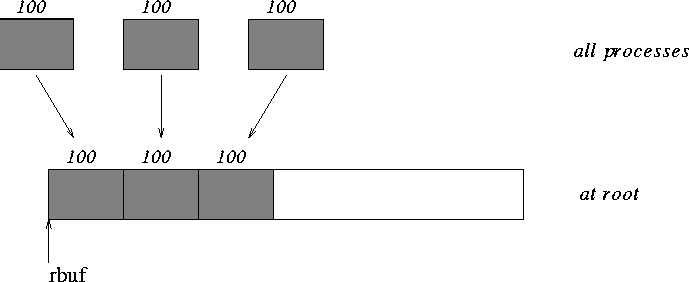
\includegraphics{imgs/mpi_gather.png}
            \caption{\texttt{MPI\_Gather}의 작동 방식\cite{MPIGather}.}\label{fig:mpi_gather}
        \end{figure}


        \textbf{통신 패턴.}
        입력 행렬 A와 같이 각 프로세스에 각기 다른 부분을 분배하는 경우, \texttt{MPI\_Scatter}를 사용하여
        한 번에 수행할 수 있다. Fig.~\ref{fig:mpi_scatter}과 같이 root에서 300개의 data를 갖고 있고
        각 프로세스에 각기 다른 100개의 data를 전달하고자 할 때, \texttt{MPI\_Scatter}를 사용하면 된다.

        입력 행렬 B와 같이 모든 프로세스에 동일한 부분을 분배하는 경우, \texttt{MPI\_Bcast}를 사용하여
        한 번에 수행할 수 있다.

        출력 행렬 C와 같이 각 프로세스가 각기 다른 부분을 갖고 있으며 이를 한 곳에 모으는 경우,
        \texttt{MPI\_Gather}를 사용하여 한 번에 수행할 수 있다. Fig.~\ref{fig:mpi_gather}과 같이
        각 프로세스가 각기 다른 100개의 data를 갖고 있고, root에서 300개의 완성된 data로 모으고자 할 때,
        \texttt{MPI\_Gather}를 사용하면 된다.

    }
    \item {
        \textbf{Strip-mining.}
        Strip-mining을 통해 액세스 패턴을 최적화하는 경우, SIMD 명령어가 다루는 데이터의 수나 프로세서가 가진
        여러 level의 캐시의 크기 등에 맞추어 연산을 분배해야 한다. 이러한 수치는 대부분 2의 지수승으로
        이루어져 있기 때문에, M, N, K의 크기가 2의 지수승이 아닌 경우 연산 루프의 마지막에 기본 단위보다
        더 작은 양을 처리하는 예외 처리 코드를 추가하거나, M, N, K의 크기를 2의 지수승으로 변환하고 추가된 부분을
        0으로 채워 재배열하는 등의 추가적인 처리가 필요하게 된다. 이러한 추가 연산은 커널 작성을 복잡하게 하고,
        성능을 저하시키는 요인이 된다. 덧붙여, 연산 병렬화의 측면에서도 코어의 수나 컴퓨팅 노드의 수 등도
        2의 지수승을 따르는 경우가 대부분이므로 비슷한 어려움을 야기한다.
    }

    
\end{itemize}